\documentclass[]{article}

% Imported Packages
%------------------------------------------------------------------------------
\usepackage{amssymb}
\usepackage{hyperref}
\hypersetup{
    colorlinks=true,
    linkcolor=blue,
    filecolor=magenta,      
    urlcolor=cyan,
    pdftitle={Overleaf Example},
    pdfpagemode=FullScreen,
}
\usepackage{amstext}
\usepackage{amsthm}
\usepackage{amsmath}
\usepackage{enumerate}
\usepackage{fancyhdr}
\usepackage[margin=1in]{geometry}
\usepackage{graphicx}
\usepackage{extarrows}
\usepackage{setspace}
%------------------------------------------------------------------------------

% Header and Footer
%------------------------------------------------------------------------------
\pagestyle{plain}  
\renewcommand\headrulewidth{0.4pt}                                      
\renewcommand\footrulewidth{0.4pt}                                    
%------------------------------------------------------------------------------

% Title Details
%------------------------------------------------------------------------------
\title{Deliverable \#3}
\author{SE 3A04: Software Design II -- Large System Design}
\date{}                               
%------------------------------------------------------------------------------

% Document
%------------------------------------------------------------------------------
\begin{document}

\maketitle	
\noindent{\bf Tutorial Number:} T01\\
{\bf Group Number:} G6 \\
{\bf Group Members:} 
\begin{itemize}
	\item Jane Klavir
	\item Nathan Luong
	\item Areez Visram
	\item Jennifer Ye
\end{itemize}

\section{Introduction}
\label{sec:introduction}
% Begin Section

The following document is dedicated to displaying various technical diagrams which fill in the various components of the system which were determined in Deliverable 2. The document shows heavily detailed state chart diagrams for every controller in the system, sequence diagrams for every use case for the system, and a detailed class diagram showing the interaction between all classes in the system.

\subsection{Purpose}
\label{sub:purpose}
% Begin SubSection
The purpose of this document is to communicate to the reader how the system will work in a visual way. The purpose of the various diagrams is to show enough detail that a reader can understand how the system will function and interact in different scenarios and in different states. The intended audience of this document are readers that come from a technical background. A reader with a technical software background would be equipped to adequately understand the various types of diagrams that are shown in this document.
% End SubSection

\subsection{System Description}
\label{sub:system_description}
% Begin SubSection
This system is an Android application which empowers the ability to book taxi carpools via a user-friendly interface. The application securely stores customer personal information such as carpool request histories, and personal data inputted by the user. The product is not self-contained since its functionality depends on Google Maps for mapping integration. The product scope mainly covers a match making functionality to match potential carpoolers together. The feature will be implemented under a centralized dispatcher which communicate with the mobile app and user’s database. Fare determination will be covered under the scope of the app, however payment processing is external to the system.
% End SubSection

\subsection{Overview}
\label{sub:overview}
% Begin SubSection
This document is organized into 4 distinct sections. The first section is an introduction to the document containing the purpose and description of the system. The second section displays 
state charts for the system. The state charts express what each of the controller classes do as the application runs. The third section displays sequence diagrams for each use case 
of the system. The sequence diagrams communicate the sequence and lifeline of various system objects as use cases occur. The fourth and final section 
contains a detailed class diagram which provides the internal details of all classes, as well as how they are connected with each other. This document also 
contains an appendix, which has a Division of Labour outlining the contributions of each team member to the document.

% End SubSection

% End Section

\section{State Charts for Controller Classes}
\label{sec:state_charts_for_controller_classes}
% Begin Section
This section should provide a state chart for each controller class for your application.
% End Section

\section{Sequence Diagrams}
\label{sec:sequence_diagrams}
% Begin Section
\subsection*{Use Case: User Creates Account}
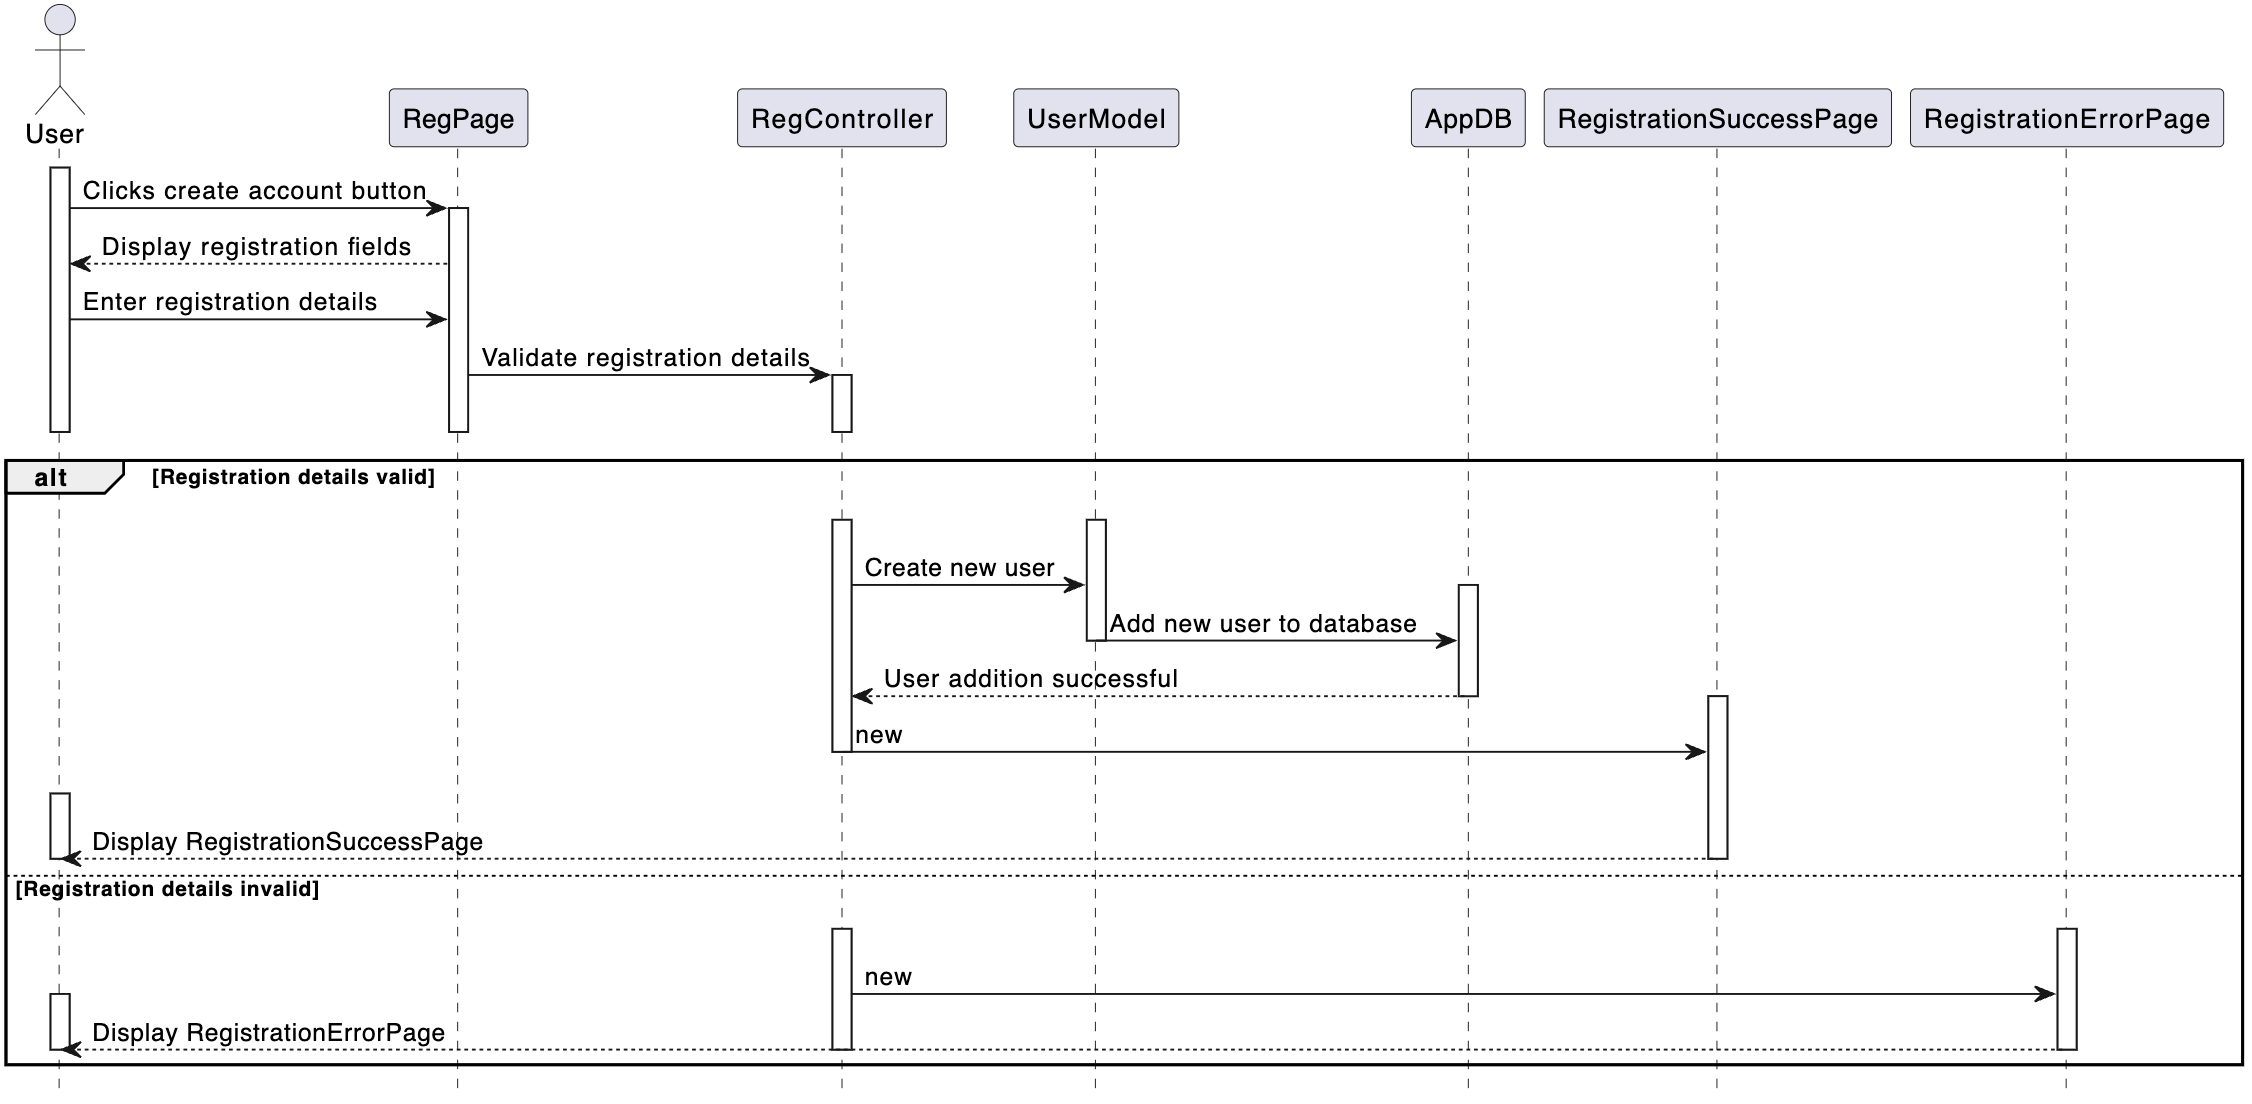
\includegraphics[scale=0.45]{Sequence Diagrams/GS1.png}

\subsection*{Use Case: User Edits Profile}
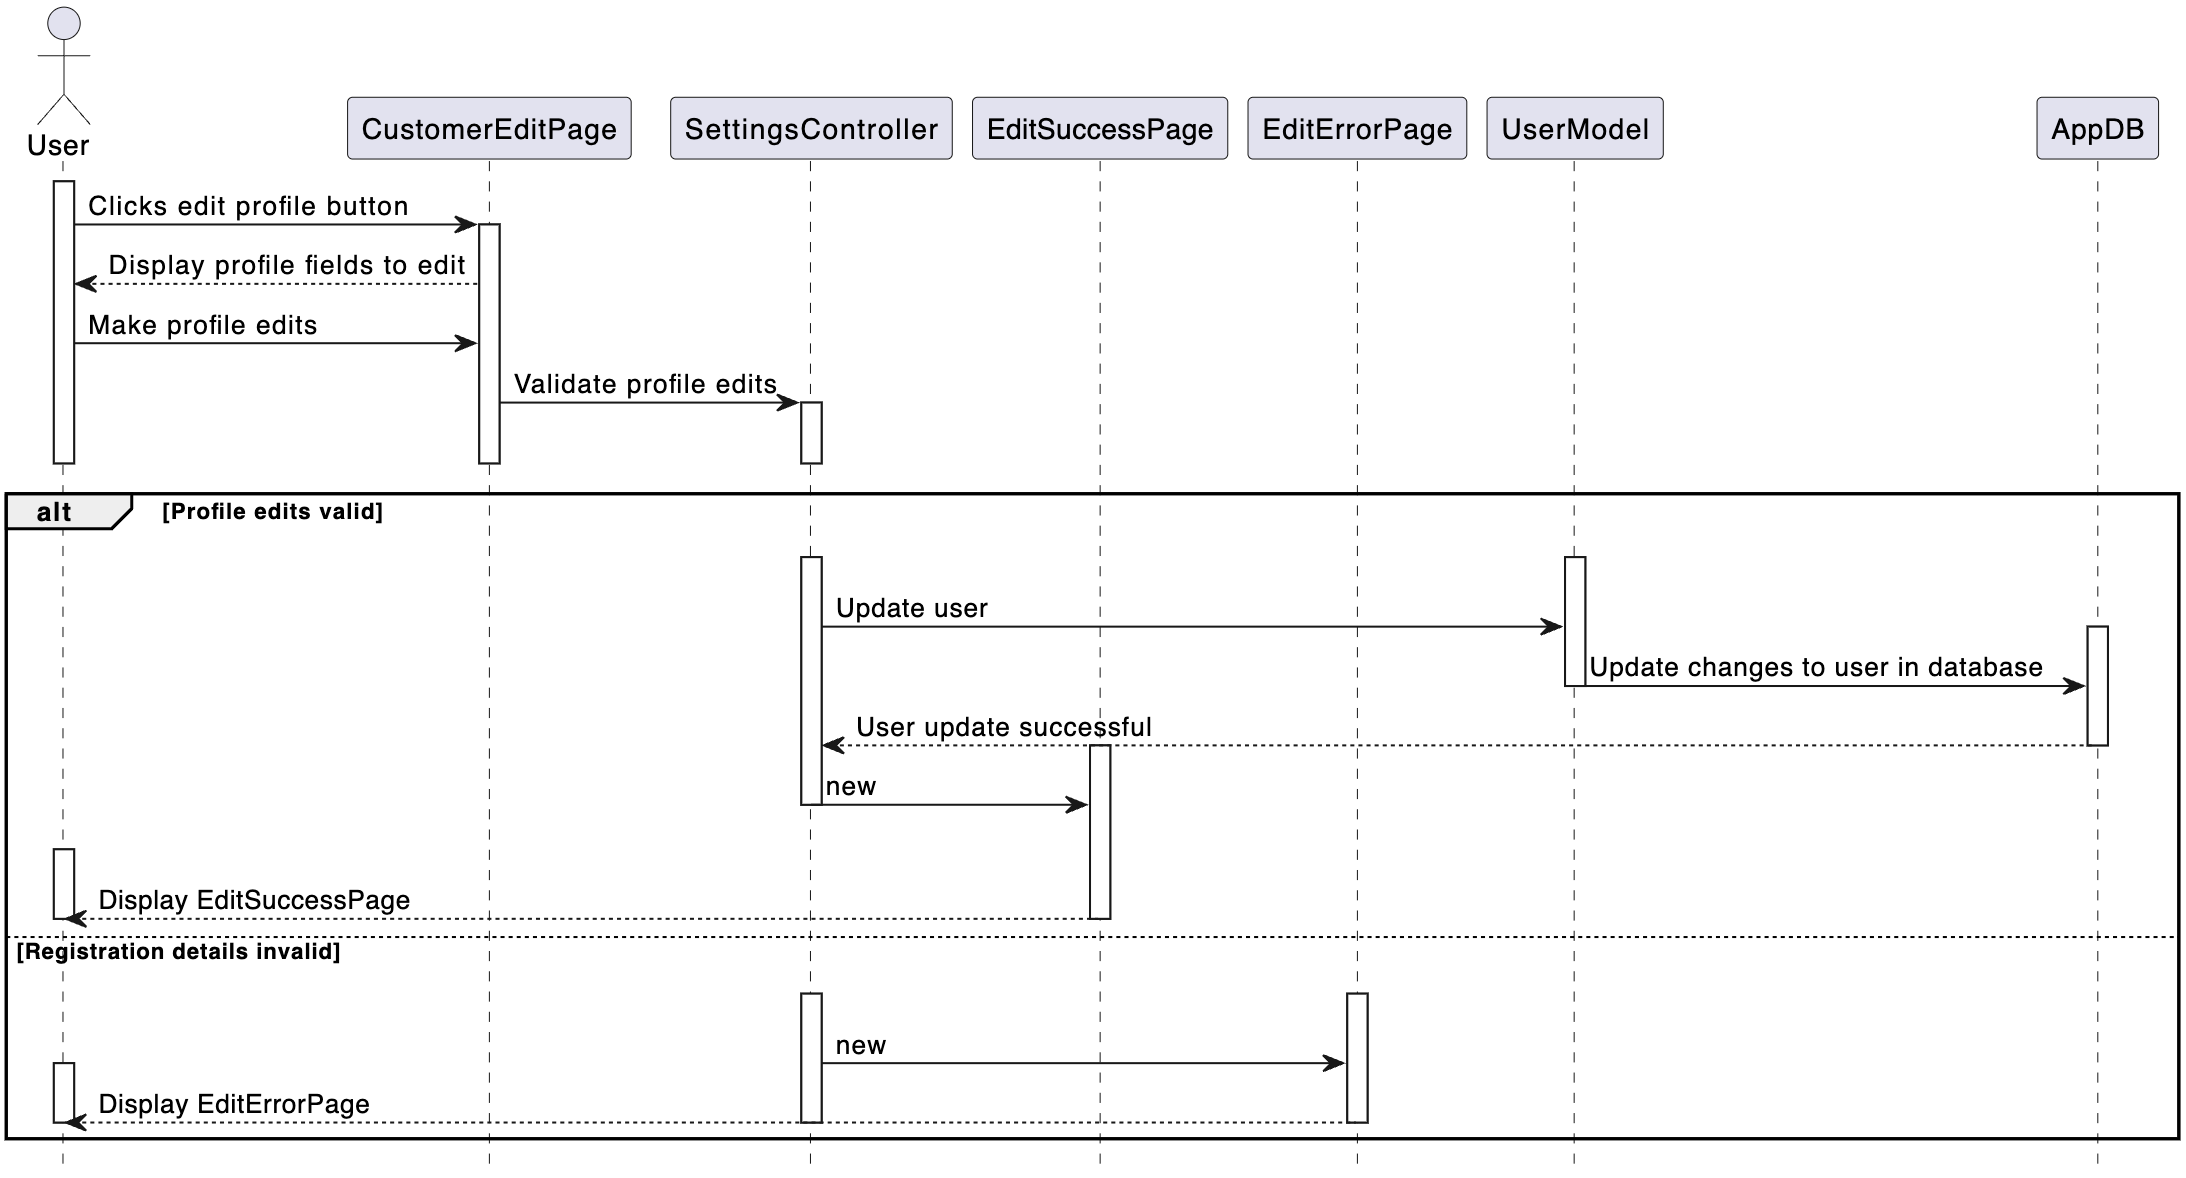
\includegraphics[scale=0.45]{Sequence Diagrams/GS2.png}

\subsection*{Use Case: User Deletes Account}
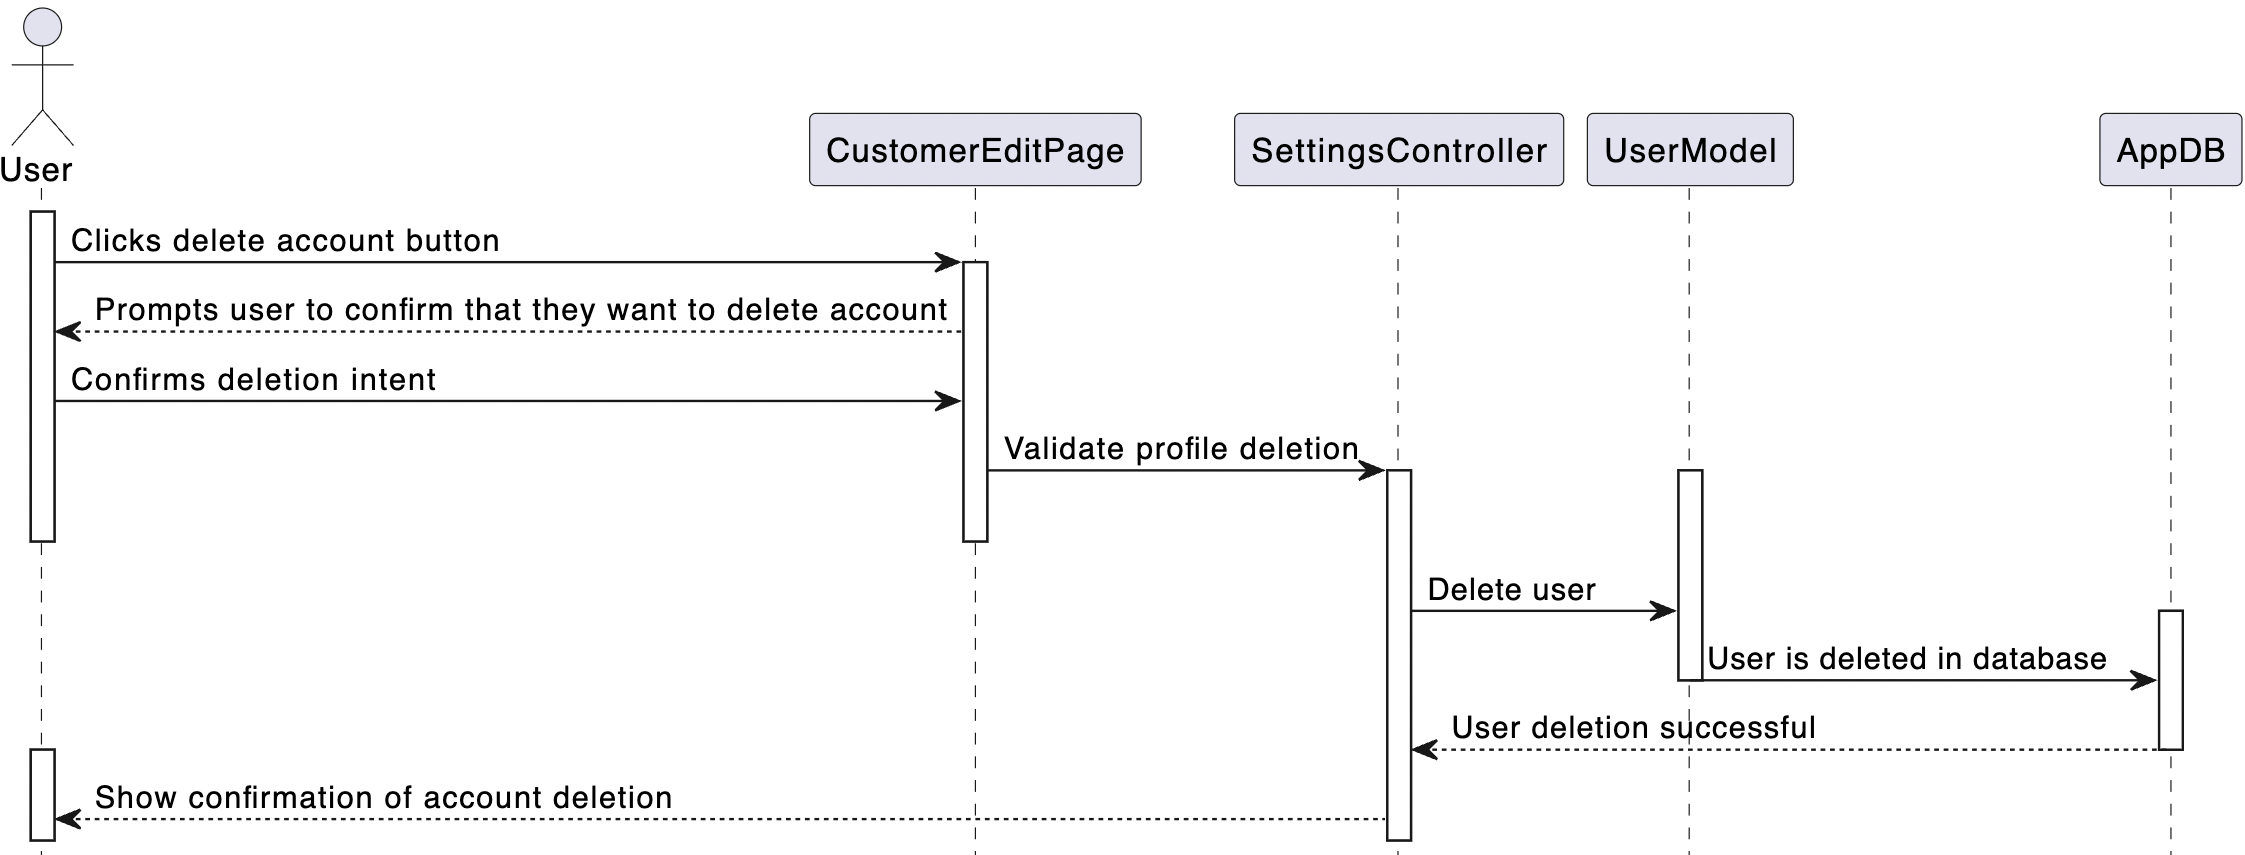
\includegraphics[scale=0.45]{Sequence Diagrams/GS3.png}

\subsection*{Use Case: Taxi Carpool is Requested}
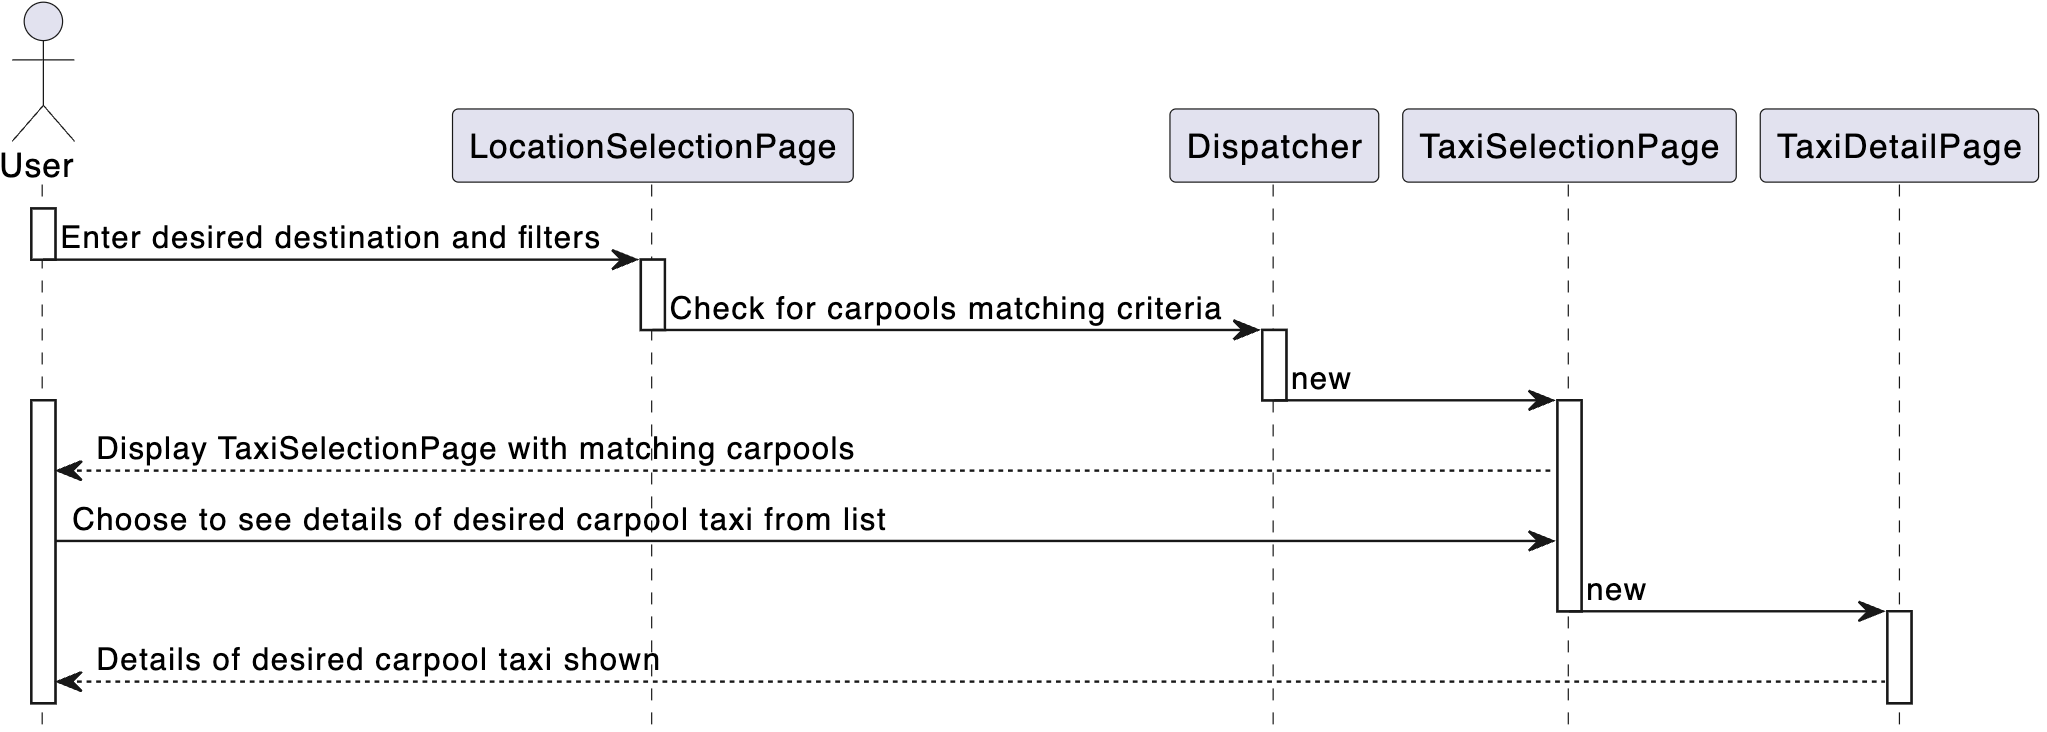
\includegraphics[scale=0.45]{Sequence Diagrams/GS4.png}

\subsection*{Use Case: Taxi Carpool is Offered}
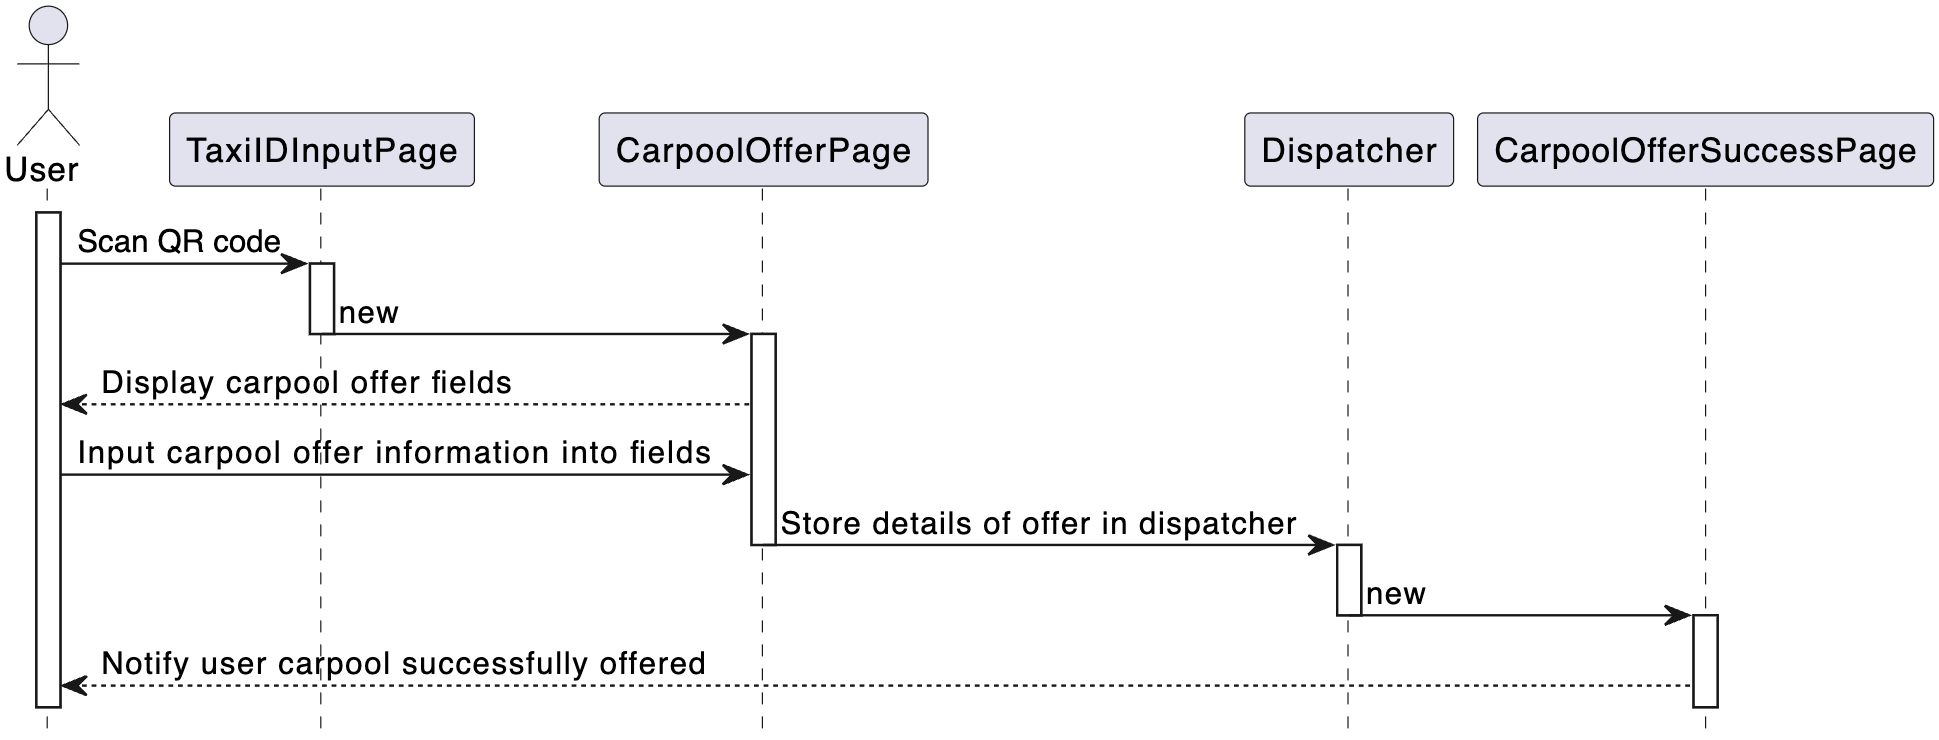
\includegraphics[scale=0.45]{Sequence Diagrams/GS5.png}

\subsection*{Use Case: Requester Chooses Match, Offerer Accepts Match}
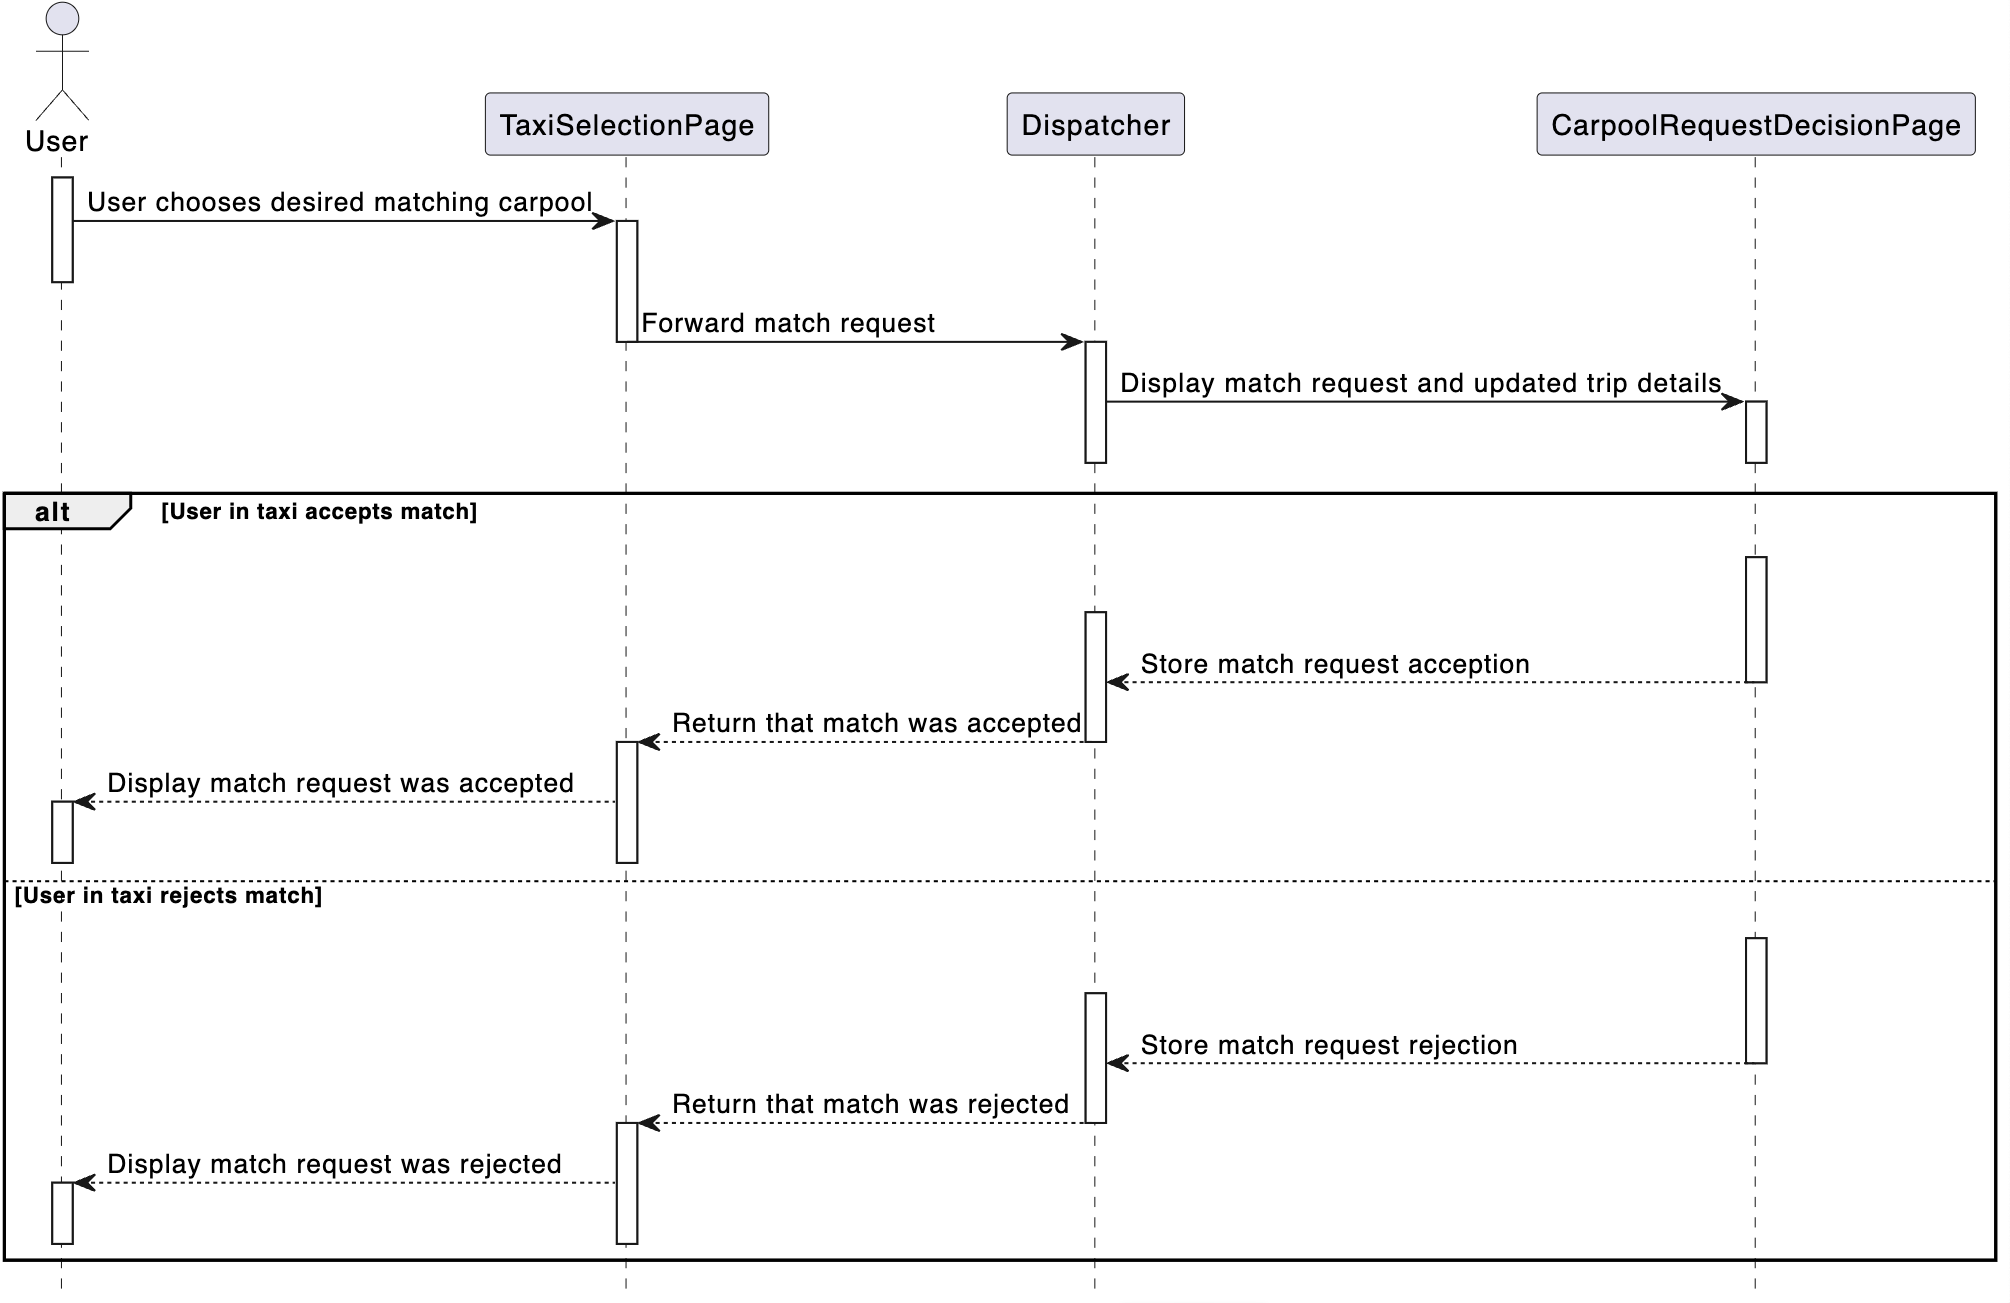
\includegraphics[scale=0.45]{Sequence Diagrams/GS8.png}

\subsection*{Use Case: Taxi Carpool Arrives at Destination}
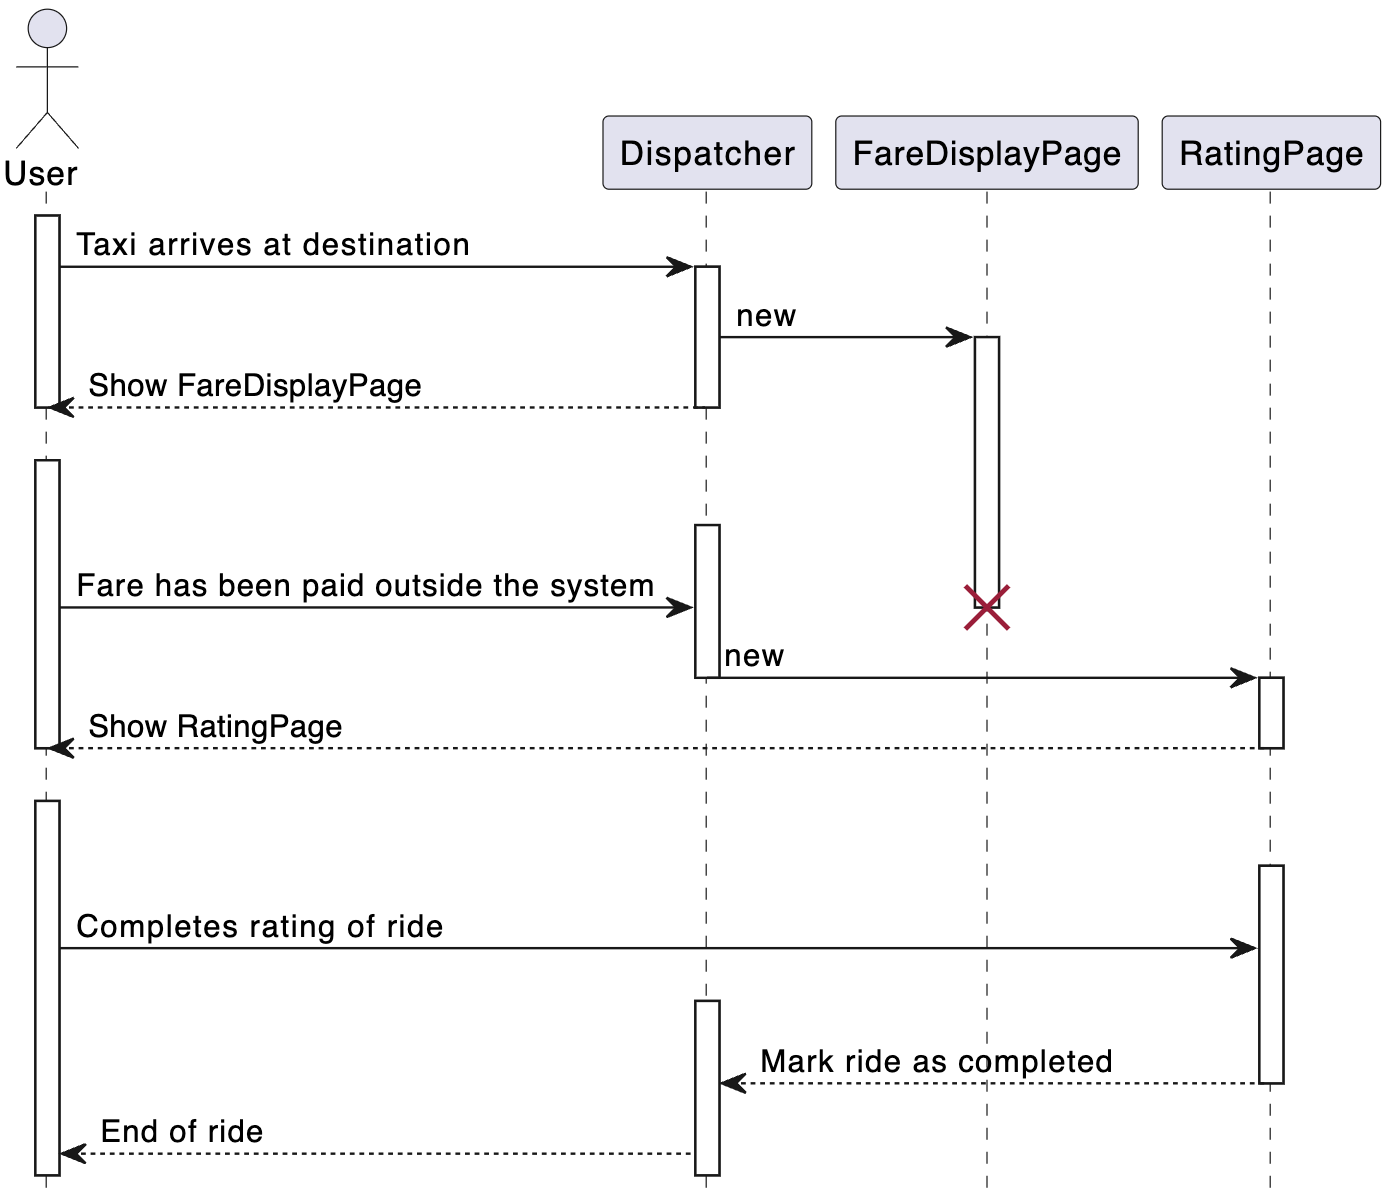
\includegraphics[scale=0.45]{Sequence Diagrams/GS6.png}

\subsection*{Use Case: Carpoolers Activate Prompts}
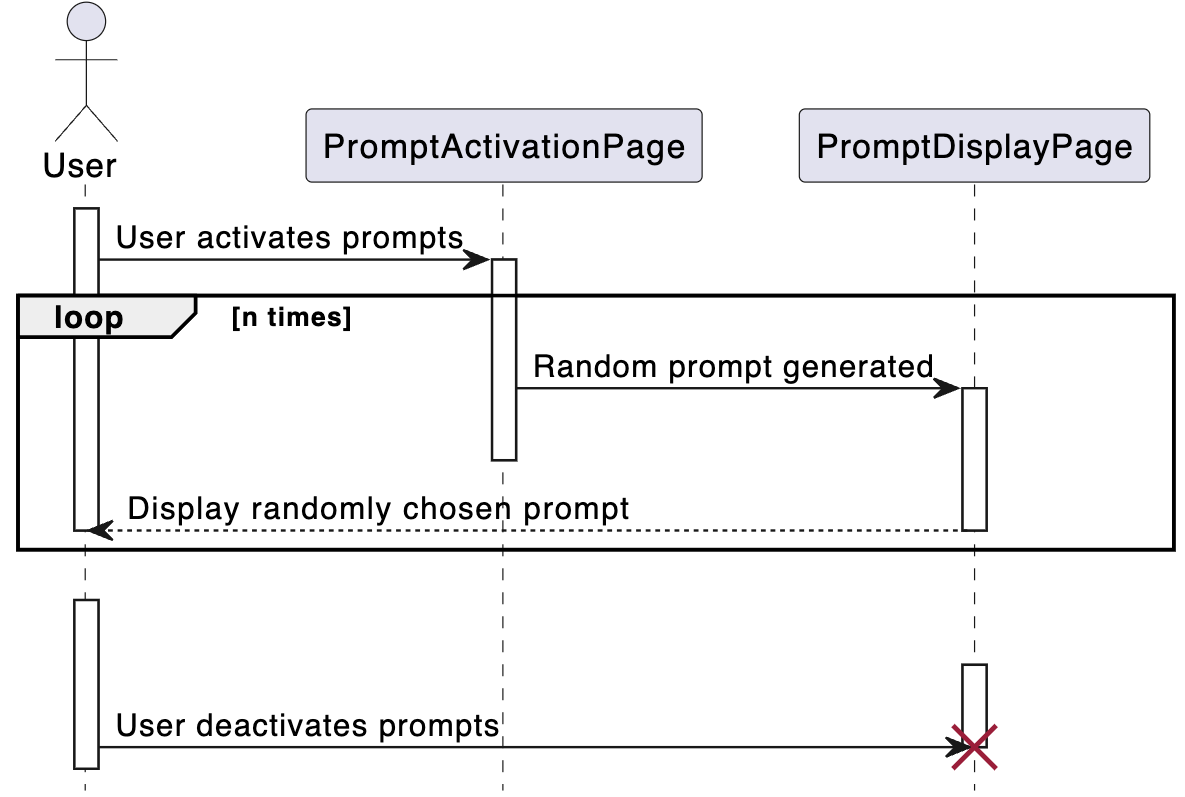
\includegraphics[scale=0.45]{Sequence Diagrams/GS7.png}
% End Section

\section{Detailed Class Diagram}
\label{sec:detailed_class_diagram}
% Begin Section
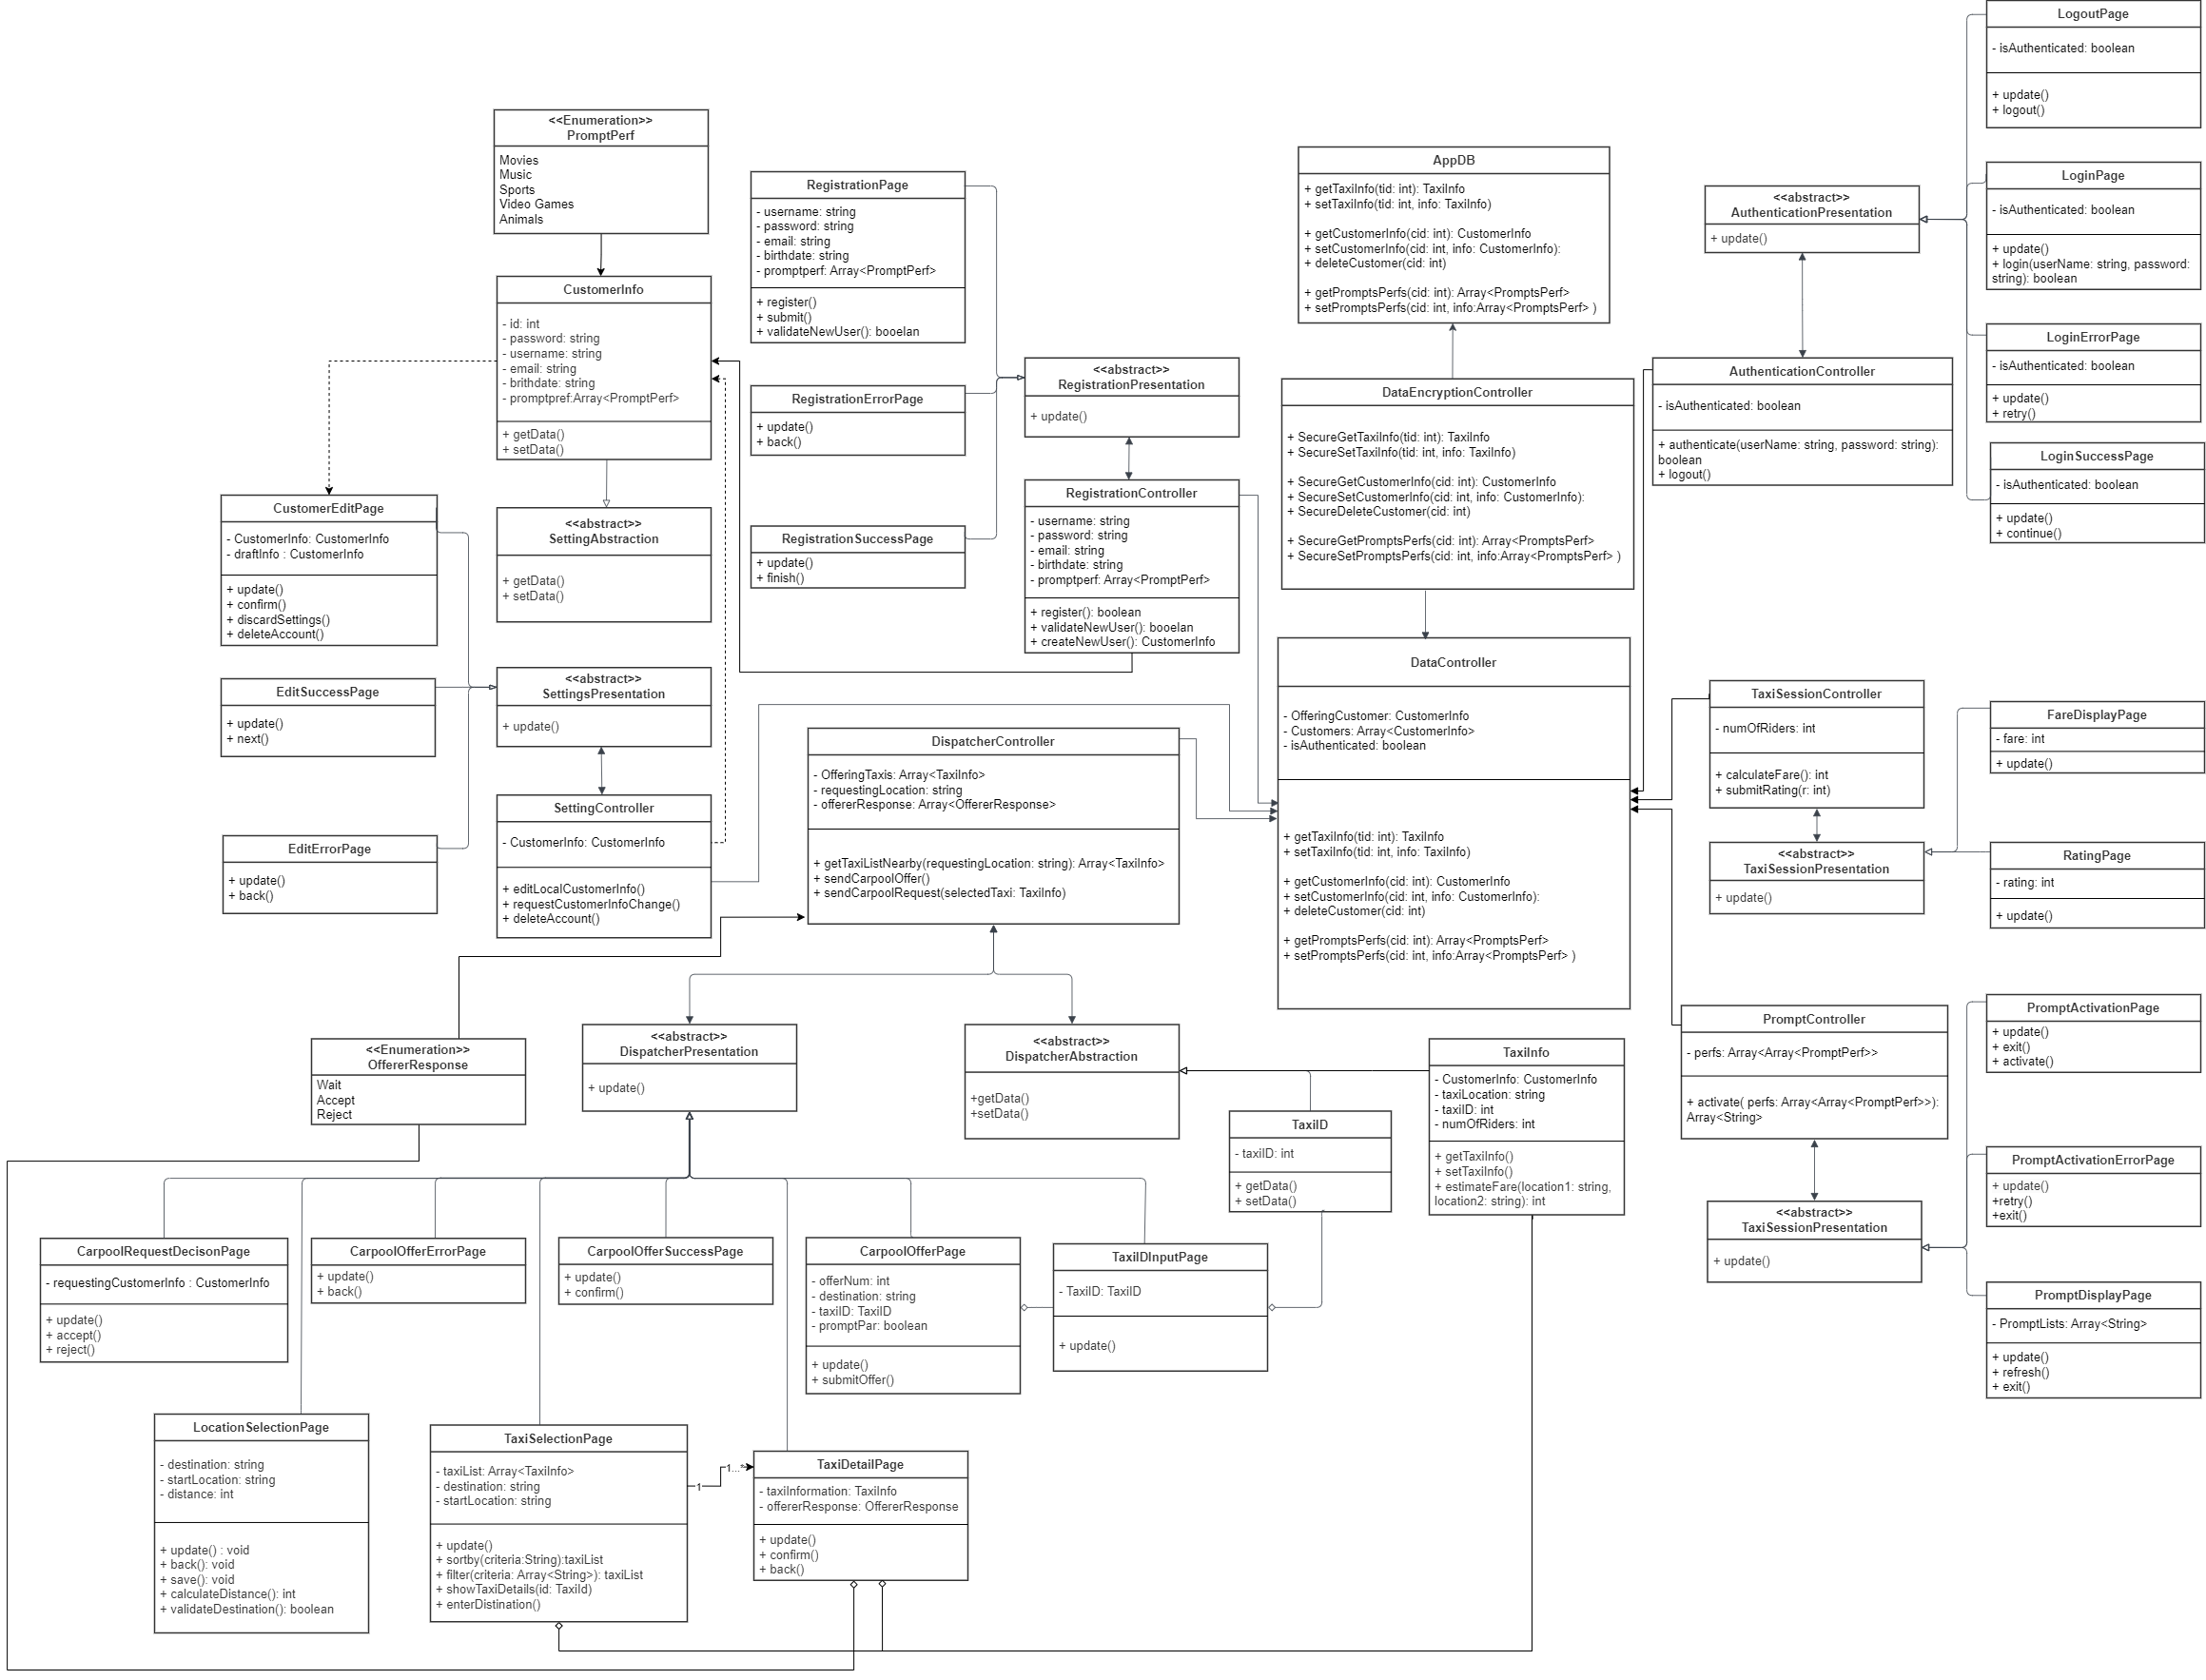
\includegraphics[scale=0.2]{images/UML-ClassDiagram.png}

The full diagram can be seen here: \href{https://cdn.discordapp.com/attachments/1065661481171038298/1087213470207967252/3A04-UML-Diagram.drawio.png}{UML Diagram Full}

% End Section

\appendix
\section{Division of Labour}
\label{sec:division_of_labour}
% Begin Section
Include a Division of Labour sheet which indicates the contributions of each team member. This sheet must be signed by all team members.
% End Section

\newpage
\section*{IMPORTANT NOTES}
\begin{itemize}
	\item You do \underline{NOT} need to provide a text explanation of each diagram; the diagram should speak for itself
	\item Please document any non-standard notations that you may have used
	\begin{itemize}
		\item \emph{Rule of Thumb}: if you feel there is any doubt surrounding the meaning of your notations, document them
	\end{itemize}
	\item Some diagrams may be difficult to fit into one page
	\begin{itemize}
		\item It is OK if the text is small but please ensure that it is readable when printed
		\item If you need to break a diagram onto multiple pages, please adopt a system of doing so and throughly explain how it can be reconnected from one page to the next; if you are unsure about this, please ask me
	\end{itemize}
	\item Please submit the latest version of Deliverable 1 and Deliverable 2 with Deliverable 3
	\begin{itemize}
		\item They do not have to be a freshly printed versions; the latest marked versions are OK
	\end{itemize}
	\item If you do \underline{NOT} have a Division of Labour sheet, your deliverable will \underline{NOT} be marked
\end{itemize}


\end{document}
%------------------------------------------------------------------------------